%!TEX root = ../thesis.tex
%*******************************************************************************
%****************************** Second Chapter *********************************
%*******************************************************************************

\chapter{Marco teórico}

\ifpdf
    \graphicspath{{Chapter2/Figs/Raster/}{Chapter2/Figs/PDF/}{Chapter2/Figs/}}
\else
    \graphicspath{{Chapter2/Figs/Vector/}{Chapter2/Figs/}}
\fi


\section{Tecnologías}

\subsection{HTTP}

HTTP, Hypertext Transfer Protocol (Protocolo de Transferencia de Hipertexto) por sus
siglas, es el protocolo por el cual se comunican navegadores, servidores y aplicaciones
relacionadas con la web alrededor de todo el mundo.

Este protocolo se encuentra en la capa de aplicación del modelo OSI. Ha estado en uso por
la World-Wide Web (WWW) desde 1990. Su primera versión hace referencia a HTTP/0.9 y era un 
protocolo simple para la transferencia de datos a través de la internet.

HTTP/1.0 surge a través de la definición del RFC 1945, este mejoró sustancialmente la
comunicación permitiendo a los mensajes encontrarse en formato MIME (Multipurpose
Internet Mail Extensions). Los servidores web adjuntan un tipo MIME a todas sus peticiones
HTTP. Cuando un navegador web obtiene una respuesta desde un servidor, mira el tipo MIME
asociado a ella para ver si sabe cómo manejar el archivo. La mayoría de los navegadores
pueden manejar cientos de tipos de archivos populares: Imágenes, videos, sonidos,
documentos de texto, entre otros.

La última versión de este procolo es la 2.0, definida en el RFC 7540 en el año 2015. Un
gran avance en esta última versión contribuye a disminuir el tráfico innecesario en 
la red definiendo un mapeo optimizado de la semántica de HTTP a una conexión subyacente.

El modo de funcionamiento es muy sencillo. Esta compuesto por dos partes quienes son 
las partes que se comunican, estas son el cliente y el servidor. Básicamente el cliente
envía peticiones al servidor y este debe servirlas en caso de poder. De lo contrario, 
el servidor devolverá el error correspondiente a alguna de las posibles causas. Algunas 
de las más comunes son que el recurso que el servidor busca no se encuentre, que el 
recurso no esté disponible, que se haya movido de lugar o que haya habido algún error 
interno.

\begin{figure}[htbp!] 
\centering    
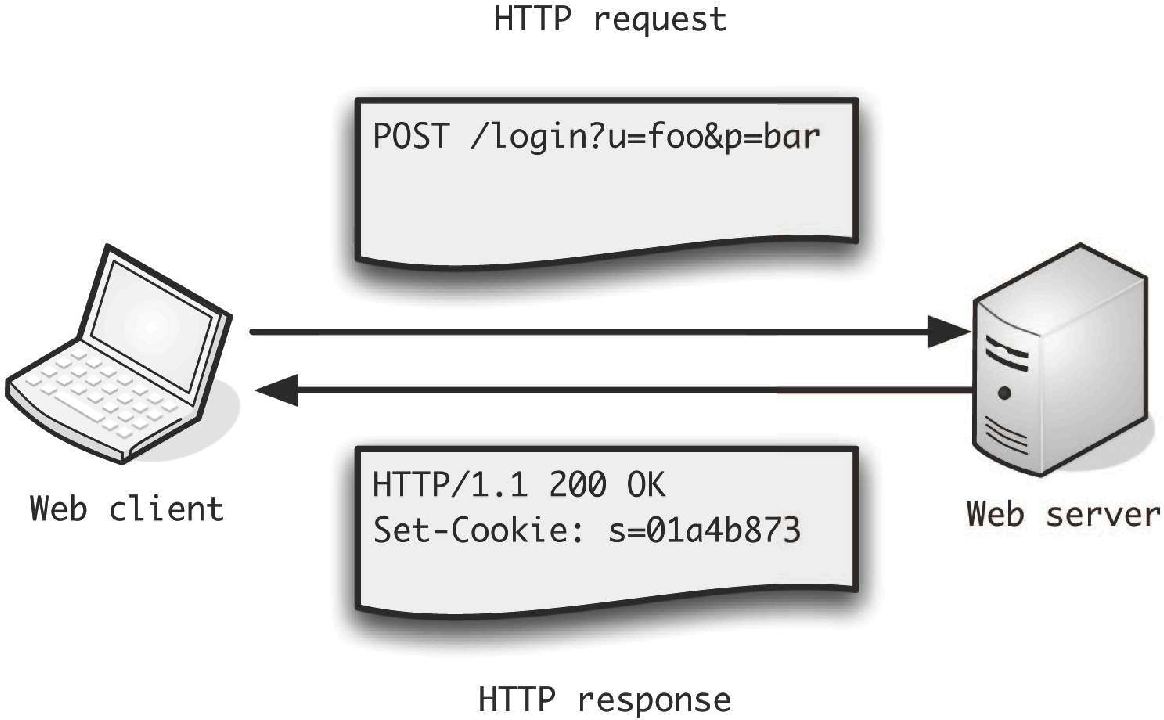
\includegraphics[width=0.5\textwidth]{http1}
\caption[HTTP]{Este es el comportamiento con información básica del protocolo HTTP}
\label{fig:http-behavior}
\end{figure}


\subsection{API REST}

La sigla REST responde a Representational State Transfer - Transferencia de Estado
Representacional. Es cualquier interfaz entre sistemas que use HTTP para obtener
datos o generar operaciones sobre esos datos en todos los formatos posibles, como XML y
JSON. También podemos decir que es un estilo de arquitectura para proveer estándares entre
sistemas de computadoras en la web. 

Su creador, Roy Fielding, es también coautor del protocolo HTTP mencionado en el capítulo 
anterior. REST nace en el año 2000.

La arquitectura REST describe seis restricciones que definen la base del estilo 
RESTful:

\begin{itemize}
   \item Interfaz Uniforme
	
	Define la interfaz entre clientes y servidores. Simplifica y desacopla la 
	arquitectura. Tiene cuatro principios:
	   
   \begin{itemize}
     \item Basada en Recursos
     
	Los recursos son identificados individualmente en las peticiones usando su URI como
	identificadores. Los recursos en si mismos están separados de lo que terminará siendo 
	su representación devuelta al cliente.     
     
     \item Manipulación de recursos a través de representaciones
     
     Cuando un cliente tiene una representación de algún recurso, esto es suficiente 
     para modificar o eliminar el recurso siempre y cuando se tenga permiso para esto.
     
     \item Mensajes auto descriptivos
     
     Cada mensaje incluye suficiente información describiendo cómo debe éste procesarse.
     
     \item Hypermedia as the Engine of Application State (HATEOAS)
     
     Los clientes entregan el estado a través del contenido del body, los parámetros de
     la query, los headers del request y el URI solicitado (el nombre del recurso). 
     Los servicios entregan estado a los clientes a través del
     body, códigos de respuesta y headers en la respuesta.
   \end{itemize}
   
	\item Sin estado
	
	Esto significa que el estado necesario para manejar la petición está contenido en 
	la petición en si misma como parte de la URI, los parámetros de la query, el body o 
	los headers. La URI identifica de manera única al recurso y el body contiene el estado 
	(o el cambio de éste) de ese recurso. Luego de que el servidor procese lo necesario, 
	la información pertinente es devuelta al cliente mediante headers, estados y el body.
	
	\item Cacheable
	
	Los clientes pueden cachear respuestas. Las respuestas deben definirse a si mismas 
	como cacheables o no cacheables. Esto es para evitar que los clientes reutilicen datos 
	inapropiados u obsoletos.
	
	\item Cliente-Servidor 
	
	La interfaz uniforme separa los clientes de los servidores. Esta separación de 
	conceptos significa que, por ejemplo, los clientes no están envueltos en el guardado 
	de datos, tarea que recae internamente en cada servidor. Por otro lado, los servidores
	no se preocupan por la interfaz de usuario o por el estado de éste. Mientras la 
	interfaz se mantenga, tanto cliente como servidor pueden ser desarrollados y/o 
	reemplazados.
	
	\item Sistema en capas
	
	Un cliente no posee la capacidad por si mismo de decir si está conectado al 
	servidor final o a un servidor intermedio. Los servidores intermedios pueden aumentar 
	la escalabilidad activando balanceadores de carga o caches compartidos.
	
	\item Código en demanda (opcional)
	
	Los servidores son temporalmente capaces de transferir al cliente funcionalidades o 
	código que éstos puedan ejecutar.

\end{itemize}


\subsubsection{Recomendaciones}

De las previas restricciones de REST nacen ciertas recomendaciones que buscan impulsar la 
efectividad y entendimiento entre sistemas.

\begin{itemize}

	\item Usar los verbos HTTP de manera que signifiquen algo
	
	Hoy en día, cualquier consumidor de APIs es capaz de enviar los verbos (HTTP) GET, 
	POST, PUT y DELETE. Estos verbos dejan bien en claro cual es la intención del request. 
	Por ejemplo, es bien sabido que un request con el vervo GET no modificará ningún 
	recurso en el servidor, sino que únicamente los solicita.
	
	\item Nombres claros en los recursos
	
	Tener nombres claros en los recursos o URIs, por ejemplo /documento/1 en lugar de 
	/api?type=documento\&id=1, mejora mucho la claridad del request. Además, los nombres 
	apropiados en los recursos nos dan un contexto del servicio mejorando el entendimiento 
	de éste. 
	
	Los nombres de los recursos deben ser sustantivos, para los verbos se utilizan los 
	verbos HTTP.
	
	\item XML y JSON
	
	No nos extenderemos demasiado en este apartado porque podríamos dedicar un capítulo 
	entero para cada uno.
	
	Se recomienda favorecer el uso de JSON por defecto aunque es bueno ofrecer ambos para 
	que el cliente elija el que desea obtener siempre y cuando los costos de implementar 
	esto no sean extravagantes.
	
	\item Considerar conectividad
	
	Uno de los principios de REST es la conectividad (mediante links hipermedia). Los 
	servicios de por si son útiles sin ellos, pero la realidad es que una API se vuelve 
	mucho mas útil, descriptiva y navegable cuando ciertos links son enviados en la 
	respuesta. Por ejemplo, en la respuesta de una API que soporta paginación en que se 
	retorna una colección de recursos, es muy útil que se retornen links para navegar 
	la paginación de la colección tales como "primer página", "última página", 
	"siguiente", "anterior".

\end{itemize}


\subsection{JWT}

JSON Web Token por sus siglas en inglés, es una forma segura de representar información 
entre dos partes. Esta manera de representar la información fue definida en el RFC 7519.

\subsubsection{¿En qué escenarios se debería usar JWT?}
\begin{itemize}
	\item Escenarios de autenticación
	
	Este es el escenario más común para usar JWT. Una vez que el usuario es logueado en el 
	sistema, cada request que se le haga luego al servidor deberá incluir el JWT, 
	permitiendo al usuario el acceso a rutas, servicios y recursos. 
	
	\item Intercambio de información
	
	JWT es una buena manera de transmitir información de manera segura entre partes. Una 
	de las causas de esto es debido a que los JWTs pueden ser firmados, se puede estar 
	seguros de que quienes envían la información son en efecto quienes dicen ser. 
\end{itemize}

\begin{figure}[htbp!] 
\centering    
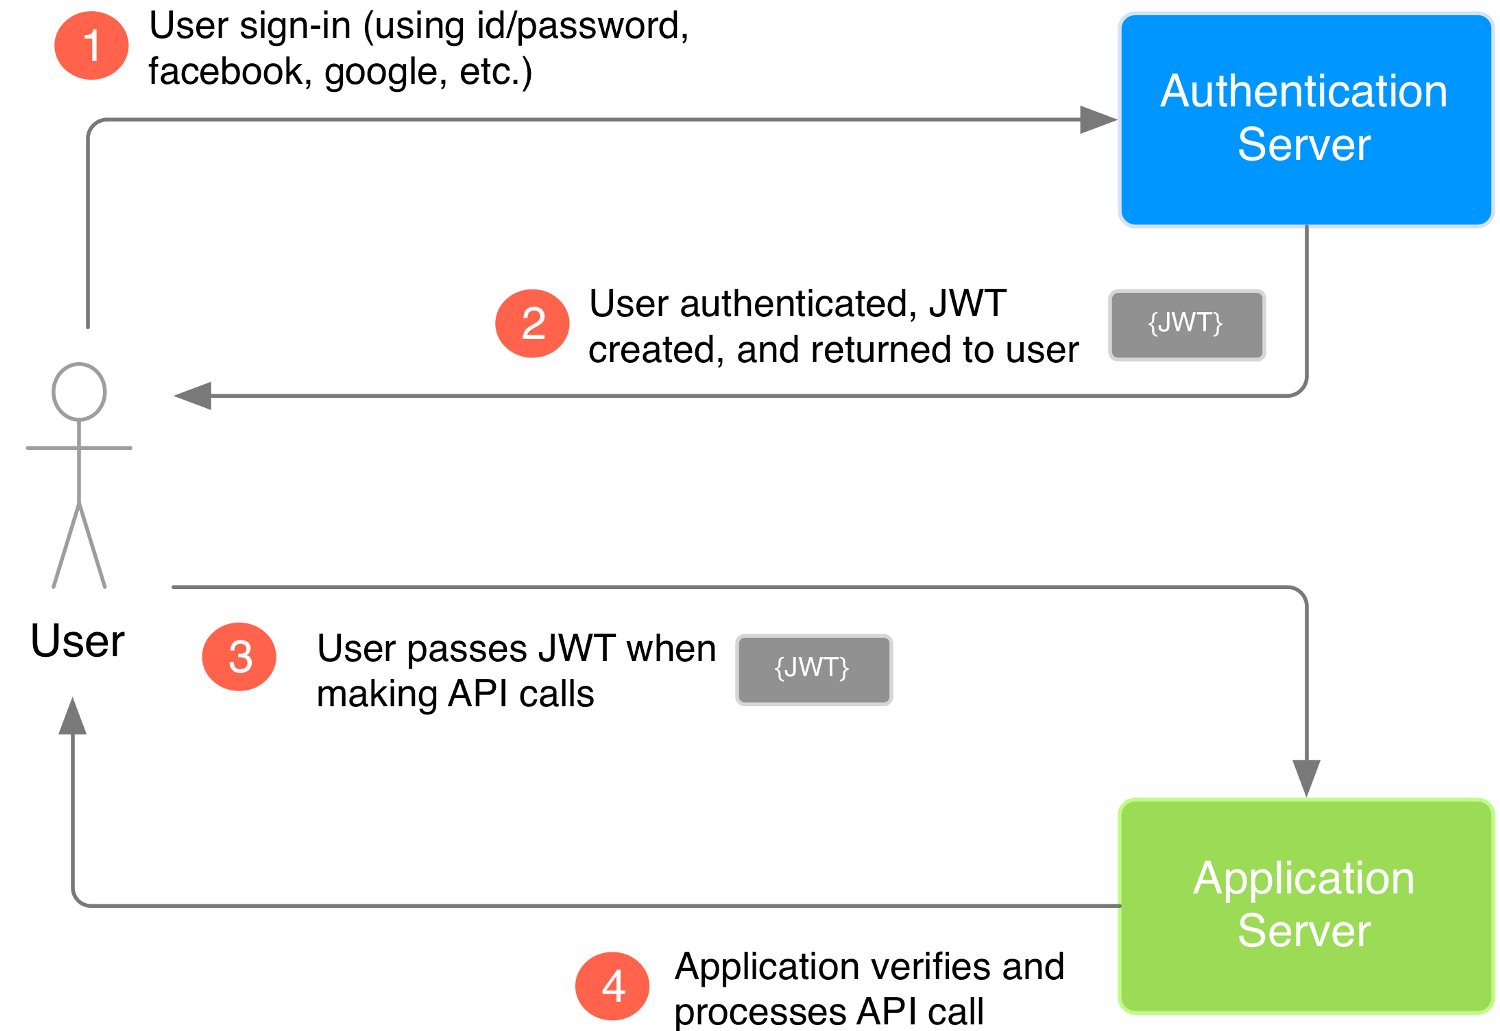
\includegraphics[width=0.6\textwidth]{jwt1}
\caption[JWT]{Como una app usa JWT para verificar la autenticidad de un usuario.}
\label{fig:jwt-auth-user}
\end{figure}

\subsubsection{Estructura del JWT}
El JSON Web Token esta formado de tres partes separadas por un punto. Comúnmente es una 
cadena de texto con el siguiente formato: header.payload.signature

\begin{itemize}
	\item Header
		
	El header del JWT contiene información sobre como debe calcularse la firma del JWT. 
	Un header es un objeto JSON con el siguiente formato:
	
	\begin{figure}[H] 
		\centering    
		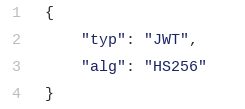
\includegraphics[width=0.3\textwidth]{jwt2}
		\caption[JWT Header]{Objeto JSON que compone el header del JWT.}
		\label{fig:jwt-header}
	\end{figure}
	
	En este JSON que compone el header, el valor de la key "typ" nos dice que el objeto 
	es un JWT y el valor de la key "alg" nos dice cual es el algoritmo de hashing para 
	crear la firma del JWT. Luego, esto se codificará usando base64.
	
	
	\item Payload
	
	En el payload del JWT vivirán los datos que queremos almacenar en este. En el siguiente 
	ejemplo, dentro del payload vivirá únicamente el id del usuario.
	
	\begin{figure}[H] 
		\centering    
		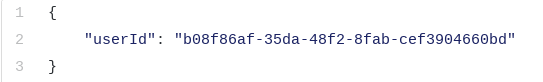
\includegraphics[width=0.5\textwidth]{jwt3}
		\caption[JWT Payload]{Datos dentro del payload. En este caso, el id de usuario.}
		\label{fig:jwt-payload}
	\end{figure}
	
	En el payload se puede guardar tanta información como se quiera. Hay que tener presente 
	que mientras mas información guardemos, más largo será el payload de nuestro token.
	
	Tal como sucede con el header, el payload es luego codificado en base64.
	
	\item Signature
	
	Para crear la firma, se debe tomar el header en base64, el payload en base64, un string 
	secreto que se utiliza para el hasheo en la encriptación y el algoritmo especificado 
	en el header bajo la key "alg". 
	
	En nuestro caso, el string resultante del header en base64 es (sin comillas) 
	"eyJ0eXAiOiJKV1QiLCJhbGciOiJIUzI1NiJ9", el payload 
	"eyJ1c2VySWQiOiJiMDhmODZhZi0zNWRhLTQ4ZjItOGZhYi1jZWYzOTA0NjYwYmQifQ", y usando como 
	string secreto, utilizaremos justamente la palabra "secret". Entonces nuestra signature 
	resultante es "\texttt{-}xN\_h82PHVTCMA9vdoHrcZxH\texttt{-}x5mb11y1537t3rGzcM".
	
	Juntando estas tres partes llegamos a tener nuestro JWT completo, este se muestra en 
	la siguiente figura.
	
	\begin{figure}[H] 
		\centering    
		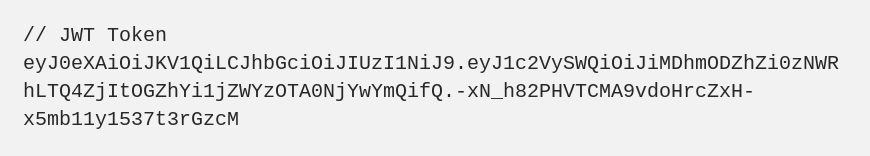
\includegraphics[width=0.5\textwidth]{jwt4}
		\caption[JWT Complete]{JWT Completo.}
		\label{fig:jwt-complete}
	\end{figure}
	
\end{itemize}

Es importante que sepamos que el propósito del JWT no es esconder ni ofuscar datos, sino 
poder probar que los datos enviados han sido generados realmente por una fuente segura.

\subsection{Memoria Cache}


\section{Herramientas y tecnologías utilizadas}

\subsection{PHP}

\subsection{Lumen Framework}

\subsection{SQL}

\subsection{Taiga}

\subsection{Vagrant}

\subsection{Git}